% This is "sig-alternate.tex" V2.0 May 2012
% This file should be compiled with V2.5 of "sig-alternate.cls" May 2012

\documentclass{sig-alternate}
\usepackage{epstopdf}
\usepackage{booktabs}
\usepackage{color, colortbl}
\usepackage{amsmath}
\usepackage{tikz}
\usetikzlibrary{arrows}

\newtheorem{problem}{Problem}
\newtheorem{definition}{Definition}
\newtheorem{pdef}{Problem Definition}
\newtheorem{theorem}{Theorem}
\newtheorem{example}{Example}
\newtheorem{obser}{{Observation}}
\newtheorem{lemma}{{Lemma}}

\DeclareMathOperator*{\argmin}{arg\,min}
\DeclareMathOperator*{\argmax}{arg\,max}


% insert graph
%\renewcommand\textfraction{}

% emphasize,terms
\newcommand{\term}[1]{{\tt#1}}

\newcommand{\Red}[1]{\textcolor[rgb]{1.00,0.00,0.00}{#1}}
\newcommand{\Blue}[1]{\textcolor[rgb]{0.00,1.00,0.00}{#1}}
\newcommand{\Green}[1]{\textcolor[rgb]{0.00,0.00,1.00}{#1}}
\newcommand{\xch}[1]{\Blue{#1}}
\newcommand{\yh}[1]{\Red{#1}}
\newcommand{\nop}[1]{}

\begin{document}

\title{Implicit Relation Inferring Using Knowledge Graph}
\subtitle{A Probabilistic Approach}

% \numberofauthors{8}

%\author{

% 1st. author
%\alignauthor
%Ben Trovato\titlenote{Dr.~Trovato insisted his name be first.}\\
%       \affaddr{Institute for Clarity in Documentation}\\
%       \affaddr{1932 Wallamaloo Lane}\\
%       \affaddr{Wallamaloo, New Zealand}\\
%       \email{trovato@corporation.com}

\maketitle
\begin{abstract}
In this paper, we propose an approach for detectiing the implicit relations between 2 entities.
\end{abstract}

%\keywords{ACM proceedings, \LaTeX, text tagging}

\section{Introduction}


Semantifying the hyperlinks in web documents is a huge task. 
Recently, more and more semi-structured documents emerge. 
There are almost hyperlinked information everywhere, but unfortunately the links lacks an explanation of why they are connected, and why human may consider them related[]. 
Specially, in Wikipedia, the relationship between entities are organized as hyperlinked entities.
%The types of hyperlink are article to article, article to knowledge base(or encyclopedia-like databases). Each link has two ends the original one(the web page/ entity page contains it) and the oriented one(the web page/ entity page it points to), and each end has 2 possible types, an anchor url or an anchor entity. Hence, in all there are 4 possible combinations, which consists the 4 type of links.
%An anchor entity can be named entities such as movies, products, people names, locations etc. In this case we explain the relation between the entity and the original article. As for an anchor url, an automatic target entity extraction process[2011] can be performed, and then it become another semantifying problem between entities.

Various tasks can benefit from semantified hyperlinks.
For machines, having the initial guess of the semantic relations can be potentially helpful. 
Many relation explanation tasks~\cite{fang2011rex,nakashole2012discovering,voskarideslearning} use semantified links in knowledge graph as input.
For semantic role labeling~\cite{palmer2010semantic} and selectional preference~\cite{pantel2007isp} and textual entailment~\cite{androutsopoulos2010survey} tasks under knowledge intensive circumstances~\cite{yao2012unsupervised,exner2011using}, knowing the semantic relationship between entities will make a differnce.
On the other hand, for readership, knowing how are the hyper-linked entities related with the source entity can be extremely helpful when sentences might sometimes be prolix and obscure.

%In this paper we focus on the problem of semantifying the first type of hyperlinks since other kinds of links can finally be deduced to this problem.

Our core idea is to utilize knowledge graph(i.e. \ac{Probase} and \ac{DBpedia}) and acquire a probabilistic distribution in concept-concept space between entity pairs for each attribute. 
For example, the relationship {\tt ArtistOf} in \ac{DBpedia} will be correct in the tuple of {\tt(Leonardo Da Vinci, artist of, Mona Lisa)} [{\tt("Human", ArtistOf, "Painting")}] and will be never correct in the tuple of {\tt ("Automobile", ArtistOf, Painting)} [e.g.{\tt(BMW i8, ArtistOf, Mona Lisa )}]. 
Then we infer which attribute would be likely to occur given a new entity pair. 

Challenges are as follows: 


We argue that the context of an entity in an article is informative[] and deserve a higher occurrence[] and can produce fresh and latest relation of an entity, which can be useful in updating the KB[reverb]. In our approach the relations is not necessarily to be exist, however the cluster of the relation[relation clustering] it belongs to should be conceptually right. With rich context and large knowledge base, we can easily derive the fresh context relations and the concept of each entity,

On the other hand, we consider the co-occurrence of the 2 entities, based on the assumption of important relationship will be observed in various of documents[]

For these reasons, we purpose a relation explanation method leveraging the concept and co-occurrence of and entity, to explain the relation between the target entity and the related entity, thus semantifying the hyperlink.

\section{Related Works}
\label{sec:rel}
%improves: incrementally training the entity-concepts so that it can model time varying attributes.(phone,manufacturer,company)--after2007-->(smartphone ,manufacturer,company)
%perform NER~\cite in the document to link the entities.
%\subsection{Relation Explanation}

Our work is closely related to the following two lines of existing efforts: relation explanation and relation extraction.

In \emph{relation explanation}, given the SPO triple of entity pairs and relationship in the knowledge graph, the goal is to retrieve text describing such relationship.
Blanco et al.~\cite{blanco2010finding} study the problem of finding support sentences to explain the relationship between a named entity and an ad-hoc query.
Fang et al.~\cite{fang2011rex} explain the relationship between 2 entities by answering a subgraph from the knowledge base.
Voskarides et al.~\cite{voskarideslearning} models the problem of explaining relationship between entities into sentences retrieval problem, ranking the explanation sentences from Wikipedia by how well it describes the relationship.
In contrast, we focus on entity pairs that do not have supporting SPO triples as input.

In \emph{relation extraction}, the goal is extracting SPO triples from text.
Early work~\cite{hearst1992automatic,brin1999extracting,agichtein2000snowball} and some wiki-based~\cite{ponzetto2008wikitaxonomy} approaches use hand-crafted patterns.
Supervised classification based works~\cite{doddington2004automatic,guodong2005exploring} are carried out on small labelled data while distant learning~\cite{craven1999constructing,wu2007autonomously,bunescu2007learning,mintz2009distant} do not require labelled data.
Recent effort~\cite{angeli2014combining} applied active learning and combines distant and partial supervision.
These efforts, including NELL, are based on fixed set of prespecified relations.
Another type of relation extraction is open relation extraction~\cite{banko2007open}, such as Reverb~\cite{fader2011identifying}, OLLIE~\cite{schmitz2012open}, which are unsupervised approaches extracting relations from plain text.
PATTY~\cite{nakashole2012patty} extract open relational patterns from Wikipedia and New York Times and organize them into a taxonomy.
Our approach is closely related to generative models, instead of the latent variables used in type-LDA model~\cite{yao2011structured}, we apply a probabilistic framework leveraging rich concepts.
Our work differs from relation extraction tasks since we are given an entity pair instead of a sentence as the input, which is more challenging.

%\subsection{Link Label Prediction}

%Link Label Prediction~\cite{agrawal2013link}

%\subsection{Information Extraction}
%
%Attribute acquisition methods
%Among domain-dependent approaches, we can mention approaches that focus on products. In this domain, attributes have been used to improve product search and recommendation [18, 22], but also to enable data mining [27]
%
%Attribute retrieval provides another granularity in Web
%search. This can interest communities that propose a more
%focused access to information or communities that envision
%aggregating pieces of information such as aggregated search
%[19, 15].


%\subsection{Link entities to Database}
%
%Linking entities to database, especially to Wikipedia, has been widely studied. Entity linking to Wikipedia~\cite{milne2008learning,mihalcea2007wikify,han2011collective} exploit Wikipedia as thesaurus and link web documents to it.
%In our work, instead of linking entities to the correspond one in KB, we extract the target entity~\cite{dalvi2011automatic} and explain the semantic relation of the entity towards target entity.


%\subsection{Short Text Conceptualization}


\section{Framework}


In this section, we present the problem and our solution to it.

\subsection{Problem Statement}

For a given pair of entity, we formalize the problem of explaining the relationship between into getting a ranking of all the possible attributes. Our target is to calculate the typicality of an attribute that can best define the possible relation of the 2 entities, which can be denoted as $P(a| (e_1,e_2) )$. One possible way is to store all the entities and their relationships, so that we can find an accurate attribute for each entity pair. Unfortunately, it is almost impossible to achieve this since there are billions of entities and new entities emerges everyday. Thus we need to utilize the concepts of the entities. Eq.~\ref{eq:target} breaks down our target into 2 parts: 1)Calculating the typicality of an attribute towards a concept pair. 2) Calculating the typicality of the concept pair towards an entity pair.
\begin{equation}
\label{eq:target}
P(a| (e_1,e_2) )= \sum_{c_1\in C_1 ,c_2 \in C_2 }P(a|(c_{1},c_{2}))\times P((c_{1},c_{2})|(e_{1},e_{2})),
\end{equation}

where $P((c_{1},c_{2})|a)$ represents the probability of given an attribute, how likely is a concept pair going to appear. 
We use Bayesian theorem to convert the first part in Eq.\ref{eq:target_expand1}:

\begin{equation}
\label{eq:target_expand1}
\begin{split}
P(a|(c_{1},c_{2})) &= \frac{ p((c_{1},c_{2})|a)\times P(a) }{ P( (c_{1},c_{2}) ) }\\
&=\frac{ p((c_{1},c_{2})|a)\times P(a) }{ \sum{P( (c_{1},c_{2})|a^* )\times P(a^*)   } },
\end{split}
\end{equation}

where $P(a)$ is defined by Eq.~\ref{eq:pa}, denoting how frequent attribute occurs.
\begin{equation}
\label{eq:pa}
P(a)=\frac{n(a)}{\sum{n(a^*)}},
\end{equation}
where $n(a)$ is the count of the attributes.

$P((c_{1},c_{2})|(e_{1},e_{2}))$ denotes the likelyhood of the occurrence a concept conbination given the entity, one naive solution is as Eq.~\ref{eq:target_expand2_naive}, following the intuition of finding typical concepts for the entity. We discuss how to calculate $P(c|e)$ for this task in detail in Section.~\ref{sec:conceptualization}.

\begin{equation}
\label{eq:target_expand2_naive}
\begin{split}
P((c_{1},c_{2})|(e_{1},e_{2})) = P(c_1|e_1) \times P(c_2|e_2)
\end{split}
\end{equation}

However, the joint distribution of the two concepts is indispensable for sense disambiguation. For example, we suppose the given entity pair is (apple, steve jobs). The potential left concepts are \term{fruit,company,...} and the right concepts are \term{entrepreneur, pc developer,...}. Obviously, we cannot combine \term{fruit} with \term{entrepreneur} in this case. Therefore, the Joint Distribution $JD(c_1,c_2)$ is introduced in Eq.~\ref{eq:target_expand2_jr}

\begin{equation}
\label{eq:target_expand2_jr}
\begin{split}
P((c_{1},c_{2})|(e_{1},e_{2})) = JD(c_1,c_2) \times P(c_1|e_1) \times P(c_2|e_2)
\end{split}
\end{equation}


Combining all these together, the complete version of $P(a|(c_{1},c_{2}))$ is described in Eq.~\ref{eq:target_expand_all}

\begin{equation}
\label{eq:target_expand_all}
\begin{split}
 P(a| (e_1,e_2) ) &= \frac{ p((c_{1},c_{2})|a)\times P(a) }{ \sum{P( (c_{1},c_{2})|a^* )\times P(a^*)   } }\\
 &\times JD(c_1,c_2) \times P(c_1|e_1) \times P(c_2|e_2)
\end{split}
\end{equation}



\subsection{Problem Solution}
Thus, the main framework is divided into 2 parts, the online part and the offline part.
\paragraph{The offline part}

According to the above derivation, there are 2 aspect we need to calculate offline: $JD(c_1,c_2)$ and $P((c_{1},c_{2})|a)$. 
We leverage the plentiful $(e_1,a,e_2)$ tuple in DBpedia and their concepts to compute




\paragraph{The online part}
For an entity pair request, we can calculate $ P(a| (e_1,e_2) )$ using Eq.~\ref{eq:target_expand_all}, where we get a typicality score for each attribute, once we get $P((c_{1},c_{2})|a)$ and $JD(c_1,c_2)$. Hence, we get a ranking of the attributes for the entity pair. 


\paragraph{Paper Orgnization}
The rest of the paper is organized as follows, Section~\ref{sec:conceptualization} describe how to derive $P(c|e)$ leveraging the \xch{basicness} of concept, Section~\ref{sec:fafa} is devoted to the offline calculation of $JD(c_1,c_2)$ and $P((c_{1},c_{2})|a)$. 

%First,we do conceptualization.
%
%Next,Judge whether the 2 entities are conceptually same
%
%Then, there are 2 cases of the CanBeExplained function:
%
%\begin{itemize}
%\item Explain 2 conceptually similar entity
%
%\begin{table}[htbp]
%  \centering
%  \caption{conceptually similar entity}
%    \begin{tabular}{rr}
%    \toprule
%    entity & concept \\
%    \midrule
%    Steve jobs & Person \\
%    Bill Gates & Person \\
%    \bottomrule
%    \end{tabular}%
%  \label{tab:addlabel}%
%\end{table}%
%
%
%\item Explain 2 conceptually different entity
%% Table generated by Excel2LaTeX from sheet 'Sheet1'
%\begin{table}[htbp]
%  \centering
%  \caption{Add caption}
%    \begin{tabular}{rr}
%    \toprule
%    entity & concept \\
%    \midrule
%    Mona Lisa & Painting \\
%    Renaissance & Period \\
%    \bottomrule
%    \end{tabular}%
%  \label{tab:addlabel}%
%\end{table}%
%
%Note that the concept here are not unique.
%
%\end{itemize}
%
%
%Last, We rank all the explanations in each step.
%
%
%

% !TEX root = main.tex
\section{Head-aware Conceptualization (Online Answering)}
\label{sec:conceptualization}
In this section, we give our solution to compute $P(c|e_i)$, the probability that $c$ is a concept of entity $e_i$ by using \ac{Probase}, a web-scale taxonomy.
As we have claimed, head-aware conceptualization is a distinguished feature of our problem.
We first motivate this problem. Then give our solution.
\nop{
We first briefly introduce Probase and give a direct solution.
However, the direct conceptualization solution ignores the unique setting of relationship explanation.
We will analyze the problems caused by our problem setting then give an improved version.
}

\nop{
\subsection{Problem Statement}

Given an entity, our target in this section is to find its rich probabilistic representation by concepts.
The \term{type} information from knowledge database such as Yago, DBpedia can be utilized to represent concepts as an option.
Nevertheless, we envision that applying probabilistic representation such as using concepts in \ac{Probase} will fit our problem better.

Probase exploit Hearst patterns to extract isA relations from 1.68 billion web pages .
For example, it extracts evidence for the claim \at{IBM \isa company, Nokia \isa company} from sentence \at{...\ac{companies} such as \ac{IBM, Nokia}...}
The core version of Probase contains 3,024,814 unique concepts, 6,768,623 unique instances, and 29,625,920 isA relations.

Given an entity $e$, from Probase, we can acquire its concepts' set $C(e)$.
For each $c_i \in C$, the frequency $n(c_i,e)$ can be accordingly derived, which means how many times the $e$ isA $c$ can be observed from the corpus.
The frequency information allows us to estimate  $P(c|e)$ by
$$P(c|e)=\frac{n(c,e)}{\sum_{c_i\in C(e)}n(c_i, e)}$$
}


\subsection{Head-aware Conceptulization}
We further state that the relationship between entities are determined by the head concepts.
For example, the \at{FoundedBy} relationship between \at{Apple Inc.} and \at{Steve Jobs} are determined by the head concepts they possessed (e.g.\ \term{company} and \term{entrepreneur}, regardless of the modifiers such as \term{technology} in the concept \term{technology company}.)
Hence, the attribute should be generated by the head concept pair instead of the concept pairs with modifiers.
This motivates us to refine the optimization objective by summing over on the head concept pairs.
Let $\bar{C}_1$ and $\bar{C}_2$ be the head concepts in  $C_1$ and $C_2$, respectively.
Our problem is refined as Eq.~\ref{eq:target_head}:
\begin{equation}
\label{eq:target_head}
\argmax_a \sum_{c_i\in \bar{C}_1 , c_j \in \bar{C}_2 } P(a|\langle c_{i},c_{j} \rangle \times P(\langle c_{i},c_{j}\rangle|\langle e_{1},e_{2}\rangle)
\end{equation}

By restricting the concept to the head concept, we can further reduce the computation cost.
The number of head concept pairs is obviously significantly smaller than that of the concept pair and that of entity pairs. 
Because most concepts are tail concepts with long modifiers.
Our statistics show that there are only 33197 head concepts, which is significantly less that 2 million original concepts.
By focusing on head concept, we effectively-yet-efficiently find the relationships without handling the huge number of long-tailed concepts and their entities.

\paragraph*{Probase}
We use Probase to do conceptualization of entities.  Probase exploit Hearst patterns to extract isA relations from 1.68 billion web pages. For example, it extracts evidence for the claim \at{IBM \isa company, Nokia \isa company} from sentence \at{...\ac{companies} such as \ac{IBM, Nokia}...}
The core version of Probase contains 3,024,814 unique concepts, 6,768,623 unique instances, and 29,625,920 isA relations.
Given an entity $e$, from Probase, we can acquire its concepts' set $C(e)$.
For each $c_i \in C$, the frequency $n(c_i,e)$ can be accordingly derived, which means how many times the $e$ isA $c$ can be observed from the corpus.
The frequency information allows us to estimate  $P(c|e)$ by
$$P(c|e)=\frac{n(c,e)}{\sum_{c_i\in C(e)}n(c_i, e)}$$

\paragraph*{Finding Head Concepts}
We use the following procedure to get head concept of an entity $e$.
We first retrieve all concepts of $e$ in Probase. Let the set of these concepts be $C(e)$.
Then, we reduce $C(e)$ to $\bar{C}(e)$ so that each concept in $\bar{C}(e)$ contains all {\bf head} concepts of each concept in $C(e)$.
We identify the head concept by syntax-based patterns~\cite{ponzetto2007deriving} for noun phrases.
We denote each head concept as $c_h$ and the concept with modifiers as $c_{l}$.
We use $\bar{C}(e)$ to denote the set of head concepts of $e$.
Our problem is reduced to the recalculation of the probability $P({c_h}|e)$.

\nop{
We report the changes of the $Probase$ concept space when applied our conceptualize method in Table~\ref{tab:nhc}.
We have 33197 head concepts after doing the head modifier detection, while 2 million concepts before, which reduce the search space of concept.
The increase of the average occurrence indicates the confidence of the $e$\isa$c$ pair is increased.
The increase of the average children per concept makes entities less unique, which will help avoid entity with same head concept share no long concept.

\begin{table}[htbp]
  \centering
  \caption{Necessity of Head Conceptualization}
    \begin{tabular}{rrrr}
    \toprule
          & Before & After & Changed\% \\
    \midrule
    concept number & 2127953 & 33197 & -98.44 \\
    average occurrence & 1.75  & 2.71  & 54.85714 \\
    children per concept & 7.53  & 184.3 & 2347.543 \\
    parents per entity & 2.33  & 1.55  & -33.4764 \\
    \bottomrule
    \end{tabular}%
  \label{tab:nhc}%
\end{table}%
}

\subsection{Conceptualization into Head Concepts}
One problem in the estimation of $p(c_h|e)$ is that we are likely to underestimate $p(c_h|e)$ because in general there is no sufficient direct isA relationships from entity $e$ to the head concept $c_h$.
We illustrate this in Example~\ref{exa:conc}. 


%For our task, we only need relatively general concepts(a.k.a. head concepts).
\begin{example}[Underestimation]
\label{exa:conc}
Consider the entity \ac{Thomas Watson}, by whom \ac{IBM} was founded. Its concepts in Probase include \ac{\{success leader,modern day entrepreneur,... \}}. The isA link from \at{Thomas Watson} to \at{entrepreneur} is however missing since we always refer to \at{Thomas Watson} as a modern day entrepreneur. The direct computation yields $P(\ac{entrepreneur}|\at{\text{Thomas Watson}})=0$, which is obviously an underestimation.
\end{example}



%\yh{in experiments, we should compare the baseline that directly use concepts instead of head concepts.}
\nop{
\begin{example}[Head concepts VS Original concepts]
\label{exa:HvsO}
Take \term{famous painting} as example. Its original concepts are \term{image, treasure}, which are reasonable but not plausible, since their occurrence are 2 and 1 respectively. However, the most plausible concept \term{painting} is not among the concepts.
\end{example}
}
%\yh{Rewrite the objective function when we only consider the head concepts}

\nop{
\paragraph{The main steps of conceptualization}
Given an entity $e$ from $Probase$, where we can get its concepts.
First we do head modifier detection based on syntax[], since the concepts in Probase all follows English grammar, this approach already produces a good result.
Next, we recalculate the probability of $P({c_h}|e)$ by aggregating the contribution from $c_l$.
The essentiality of doing so is illustrated in Example~\ref{exa:recalc}.
Finally, we provide a method to take the original isA relation from Probase into consideration.

\begin{example}[Essentiality of Aggregation]
\label{exa:recalc}
\term{Steve Jobs} The concept \term{well-known name} has four occurrences however \term{name} has only 2. There are other modifiers for the same head, so that the typicality of the head will be largely underestimated.
\end{example}
}

\subsection{Baseline}
The underestimation is caused by the ignorance of mentions of a entity as an instance of modified concepts. As shown in Example~\ref{exa:clc}, we should counts the number that $e$ isA $c_{l}$ when we count the $e$ isA $c_{h}$ for any $c_l$ that is a modified concept of $c_h$.
Hence, the most straight forward approach is rectifying the $n(e, c_h)$ by the additionally counting 
all $n(e, c_l)$ such that $h(c_l)=c_h$, where $h()$ is a function that generate the head concept of a long concept. The rectification is shown in Eq~\ref{eq:rec}. According to the rectified count, we have a rectified estimation on $P(c_h|e)$, as shown in Eq~\ref{eq:recp}.
\begin{equation}
\hat{n}(c_h, e)={n}(c_h, e)+\sum_{ h(c_l)=c_h} n(c_l,e)
\label{eq:rec}
\end{equation}

\begin{equation}
\hat{P}(c_h|e)=\frac{\hat{n}(c_h, e)}{\sum_{c_{h'}}{\hat{n}(c_{h'}}, e)}
\label{eq:recp}
\end{equation}

\begin{example}[Rectification by Modified Concepts]
\label{exa:clc}
As illustrated in Figure~\ref{fig:pgge}, in Probase, \at{Bill Gates} isA  \at{Leader} and \at{Bill Gates} isA \at{Business Leader} are observed respectively 9 times and 17 times from corpus. Since \at{Business Leader} is always a \at{Leader},  logically, \at{Bill Gates} isA \at{Leader} was observed 26 times instead of 9 times.
\end{example}


\subsection{Improvement by Concepts with Different Heads}
Except the modified concepts of a head, there are some other concepts that has different heads but  are semantically subclasses of the head concept. These subconcepts should be taken into account to estimate the ${P}(c_h|e)$.  We illustrate the rationality in Example.~\ref{exa:isagood}.

\begin{example}[Concepts with Different Heads]
\label{exa:isagood}
For example in Figure~\ref{fig:pgge}, \at{Bill Gates} has isA links to \at{successful entrepreneur} and \at{Industry Leader}. These two concepts has isA links to \at{business leader} and \at{Industry Leader}, respectively.  which is reasonable. Although these two concepts are not the modified concepts of \at{Leader}, their mentions as a concept of \at{Bill Gates}  should be considered when estimating $P(\at{Leader}|\at{Bill Gates})$.
\end{example}

\begin{figure}[!hptb]
\label{fig:pgge}
\centering
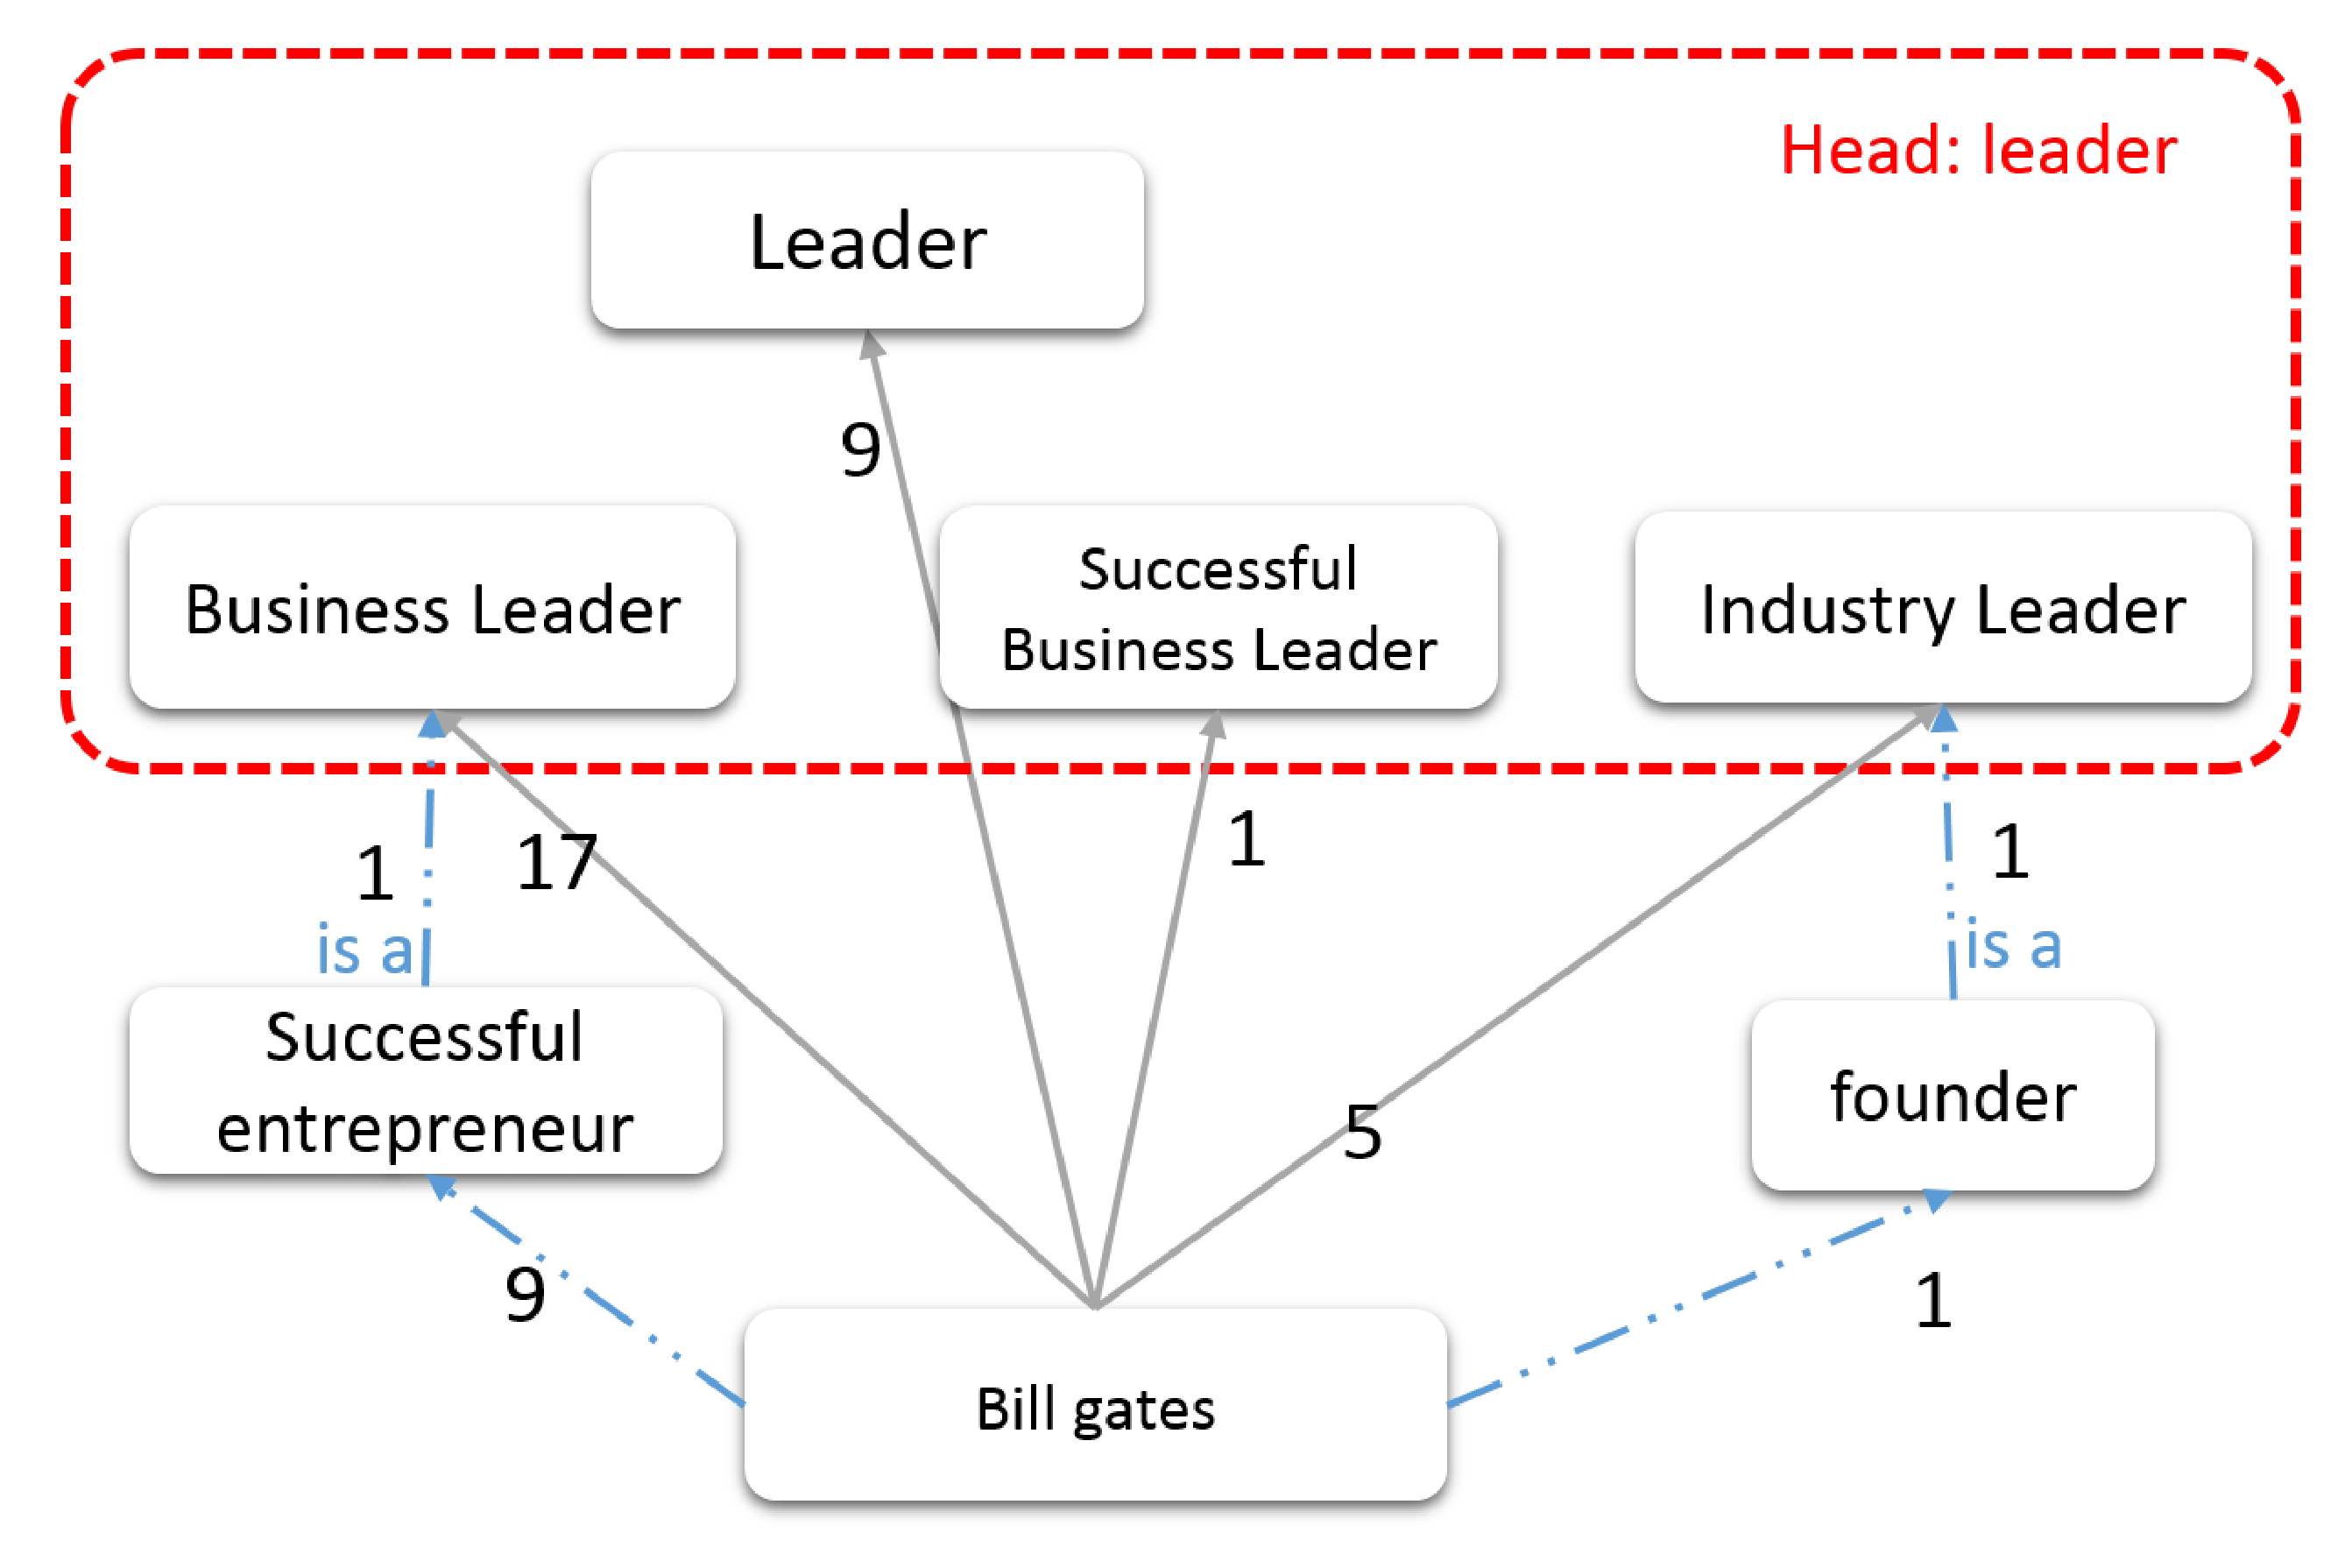
\epsfig{file=resources/bill_gates_isa.eps,width=\columnwidth}%5.5in
%考虑 transitivity: e \isa $c_l$ \isa $c_h$,  e \isa $c_l$* transitivity_coeff(cl->ch) = e \isa ch
\caption{calculating $P({c}|\term{Bill Gates})$ }
\end{figure}

%%%%%%%%%%%%%%%%%%%%%%%%%%%%%%%%%%
%\nop{
%In both case B.1 and B.2, the weight of the edge $c_{l}$ \isa ${c_h}$ is underestimated. We argue that when calculating the typicality $P({c_h}|e)$, the counts of the long concept contributing to its head concept should be re-estimated as follows.
%
%Notice that the boundary between case B.1 and case B.2 are not strict, there are such edges that have low observation in Example~\ref{exa:HvsO}. So that if we consider them as a whole, we can derive:
%\begin{equation} P({c_h}|c_{l})=\lambda P_{head}({c_h}|c_{l})+(1-\lambda)P_{probase}({c_h}|c_{l}) \label{eq:pcgclong}\end{equation}
%where $\lambda$ is a parameter \xch{principle: related to plausibility, number of occurrence, varies for different $c_{l}$ should it be derived from learning ?} since we assume $P_{head}({c_h}|c_{l})$ to be 1, Eq.~\ref{eq:pcgclong} is simplified to:
%$$P({c_h}|c_{l})=\lambda  +(1-\lambda)P_{probase}({c_h}|c_{l}) $$
%}
%%%%%%%%%%%%%%%%%%%%%%%%%%%%%%%%%%%%
Now we elaborate how to take into account the subconcepts with different heads. We first argue that we can not directly count its number of isA mentions like Eq~\ref{eq:rec}. Because its mentions should be contributed to its own head. For example, for \at{successful entrepreneur}, the number of \at{Bill Gates} isA \at{successful entrepreneur} should be attributed to \at{entrepreneur} instead of \at{Leader}.
Hence, we need a new framework. 

Instead of direct lying rectifying the isA count, we rectify the conditional probability in Eq.~\ref{eq:recp} by counting additional probability contributed by subconcepts with different heads. Given an entity $e$ and one of its head concept $h$, let $C_h$ be the set of all $h$'s modified concepts and $h$ itself. let $C^*_h$ be all concepts with different head but has a isA link to one concept in $C_h$. We can quantify how likely an entity $e$ reaches to any one concept in $C_h$ by a random walk process. In the random walk procedure, we use $P(c|e)=\frac{n(c,e)}{n(e)}$ as the random walk probability from $e$ to $c$. We can similarly define $P(c_1|c_2)$ when $c_2$ is a subconcept of $c_1$.  Thus, we need to aggregate all the random walk probability from $e$ to any concept in $C_h$.
Hence, our improved estimation of $P({c_h}|e)$ is as follows:

\begin{equation}
\hat{P}({c_h}|e) = \gamma \hat{P}({c_h}|e)+ (1-\gamma) \sum_{c_i\in C^*_h}\sum_{ c_j\in C_h} P(c_j|c_i) P(c_i|e)
\label{eq:pgge}
\end{equation}
where we use $\gamma$ to tune relative importance of two parts and $1-\gamma$ part is the contribution from the subconcept with different heads.


Note that we only consider two-steps of random walk due to the following reasons. 
First, long-steps random walk tend to introduce two general or non-realted concepts such as \term{issue, factor, element}, which are concepts for almost everything.
Second, long steps random walk in general is costly since most real graphs are small-world.
%bill gates 的例子OK 么, 如果OK 我开始写example of calculation

%
%The process of calculation is illustrated in the example~\ref{exa:calc}
%
%\begin{example}[Calculating $P({c_h}|e)$]
%\label{exa:calc}
%As illustrated in Fig.~\ref{fig:pgge}, the process of calculating the typicality a concept is as follows, where \term{painting} is ${c_h}$ and \term{Mona Lisa} is $e$. Then $P(\term{painting}|\term{Mona Lisa})$ consists of 2 parts, the direct edge $P_{original}({c_h}|e)= 0.23$, and the second part
%$$\sum_{ c_{l}^*\in C_{l} } [ \lambda_{i}^*+(\alpha_{i}^*) P({c_h}|c_{l}^*) ] \times  P(c_{l}^*|e) $$
%$(\alpha_i^*+{c_h}^*=1)$
%Thus we get
%$$ P = 0.007\times \lambda_{i2}+0.05\times \lambda_{i1}+0.04\times(\lambda_{i3}+0.65\alpha_{i3}) $$
%For \term{piece}, it is the similar process. The relation here is only part of the whole graph.
%\end{example}

%\begin{tikzpicture}[->,>=stealth',shorten >=1pt,auto,node distance= 3 cm,
%  thick,main node/.style={circle,fill=blue!10,draw,font=\sffamily\bfseries,align = center}]
%
%  \node[main node] (4) {piece};
%  \node[main node] (2) [left of=4] {painting};
%
%  \node[main node] (5) [below of=2] {oil painting};
%  \node[main node] (6) [left of=5] {famous\\painting};
%  \node[main node] (7) [left of=6] {world's\\most famous\\painting};
%
%  \node[main node] (10) [right of=5] {art piece};
%  \node[main node] (11) [right of=10] {historical\\art piece};
%
%  \node[main node] (12) [below of=6] {Mona lisa};
%
%
%  \path[every node/.style={font=\sffamily\small}]
%
%    (5) edge  node [left] {$\lambda_{i3}$} (2)
%        edge [bend right] node [right] {\small{$ 0.65\alpha_{i3} $}} (2)
%        edge  [bend right] node[left]  {\small{$ 0.28\alpha_{i3} $}} (4)
%    (6) edge [bend left] node [right] {$\lambda_{i1}$} (2)
%    (7) edge [bend left] node [right] {$\lambda_{i2}$} (2)
%
%    (10) edge [bend right] node[right] {$\lambda_{i4}$} (4)
%    (11) edge node[right] {$\lambda_{i5}$} (4)
%    (12) edge [bend right]node[right] {0.01} (10)
%         edge [bend right]node[right] {0.007} (11)
%         edge node[right] {0.04} (5)
%         edge node[right] {0.05} (6)
%         edge node[right] {0.007} (7)
%         edge node[left] {0.23} (2)
%         edge [bend right]node[right] {0.04} (4);
%
%\end{tikzpicture}

\section{Find Alias For Attributes}


argmax

% !TEX root = main.tex

\section{Experiments}
\label{sec:exp}

In this section, we present our experimental study.
We use DBpedia2014~\cite{dbpedia} and Probase~\cite{wu2012probase} as our knowledge repository.
We use entity pair as well as their attributes in DBpedia to learn the conceptual patterns.
We Probase for conceptualization. We carry out all the experiments on a PC with Intel i7 cpu @2.5Ghz and 16G memory.
All the programs implemented in Python 2.7.

\paragraph*{Evaluation Metrics}
Given two entities, our system produce the most plausible top-K attributes between the 2 entities.
We want to evaluate how accurate the result is. 
Hence we use $nDCG@K$ and $Precision@K$ as our evaluation metric.
We report the $MAP@K$ (Mean Average Precision at K) as well.
We further use $ ERR@K$~\cite{chapelle2009expected} to evaluate the Expected Reciprocal Rank, which is based on the user behavioral model emulating that user would stop browsing if the first several ranked results are undesirable.
In our collective conceptulization process, evaluating the correctness of first K concept pair $C-C$ space is similar to the user browsing case, where we can stop looking at more concepts if topK concepts already provide sufficient conceptual information for the entity pair.
% 我突然想到了我这里做过个优化, 每次算concept pairs 的时候按照P(C|E)排个序,如果排在后面的c,乘上最大的P(<c1,c2>|a)P(a)也不能超过前面的,就停止搜索了。2015年9月15日19:23:27


\subsection{Exp1: Effectiveness of $ERF$}
In this subsection, we evaluate the effectiveness of our ERF system.
For comparison, we use the direct retrieval as a baseline.
We randomly select 50 Wikipedia article, and take only the hyper-linked entities abstract part as evaluation.
We consider the linked entities as the $e_2$ of the relation explanation input and source entity as $e_1$.
Compared with baseline, i.e. DBpedia original.
Since we assume 0 if the entity has no relation can be retrieved from database and otherwise 1, the average $Precision@1$ results here can also be viewed as \ac{recall} of the knowledge base.
DBpedia provides only one relation for a covered entity pair, therefore we use $Precision@1$ to compare the results.
Our ERF method improves the average $Precision@1$ by 15.77\%.
The result is reported in Table~\ref{tab:precision_compare}

\begin{table}[htbp]
  \centering
  \caption{Precision@1 Compared With Baseline}
    \begin{tabular}{rrr}
    \toprule
         & P@1  & \%Improv. \\
    \midrule
    Dbpedia direct & 0.64 & -- \\
    ERF  & 0.83 & 15.77 \\
    \bottomrule
    \end{tabular}%
  \label{tab:precision_compare}%
\end{table}%


To further justify the effectiveness of $ERF$, we compare the overall results against baseline(no head ....).
  We report all the precision metrics in Table~\ref{tab:ndcg}.

\begin{table}[htbp]
  \centering
  \caption{Evaluation Result}
    \begin{tabular}{rr}
    \toprule
    mesure & value \\
    \midrule
    nDCG@3 & 0.945 \\
    nDCG@5 & 0.941 \\
    precision@3 & 0.88 \\
    precision@5 & 0.76 \\
    MAP@3 & 0.902 \\
    MAP@5 & 0.907 \\

    \bottomrule
    \end{tabular}%
  \label{tab:ndcg}%
\end{table}%





\subsection{Exp 2: Head-aware Conceptualization}
In this experiment, we show that head-aware conceptualization significantly reduce the computation cost without sacrificing precision. 
In Table~\ref{tab:nhc}, we report the changes of the $Probase$ concept space when applied our conceptualize method, where we have 33197 head concepts after doing the head modifier detection, while 2 million concepts before.

The increase of the average occurrence indicates the confidence of the $e$\isa$c$ pair is increased.
The increase of the average children per concept makes entities less unique, which will help avoid entity with same head concept share no long concept.

\begin{table}[htbp]
  \centering
  \caption{Necessity of Head Conceptualization}
    \begin{tabular}{rrrr}
    \toprule
          & Before & After & Changed\% \\
    \midrule
    concept number & 2127953 & 33197 & -98.44 \\
    average occurrence & 1.75  & 2.71  & 54.85714 \\
    children per concept & 7.53  & 184.3 & 2347.543 \\
    parents per entity & 2.33  & 1.55  & -33.4764 \\
    \bottomrule
    \end{tabular}%
  \label{tab:nhc}%
\end{table}%


We give the distribution comparison of head aggregation and original Probase to show the underestimation of concepts.
Figure~\ref{fig:hac} illustrate the distribution, from which we can observe that head-aware conceptualization aggregate the piecemeal long concepts to provide an estimation in a smaller concept space without losing the accuracy.


\begin{figure}[!htb]
\centering
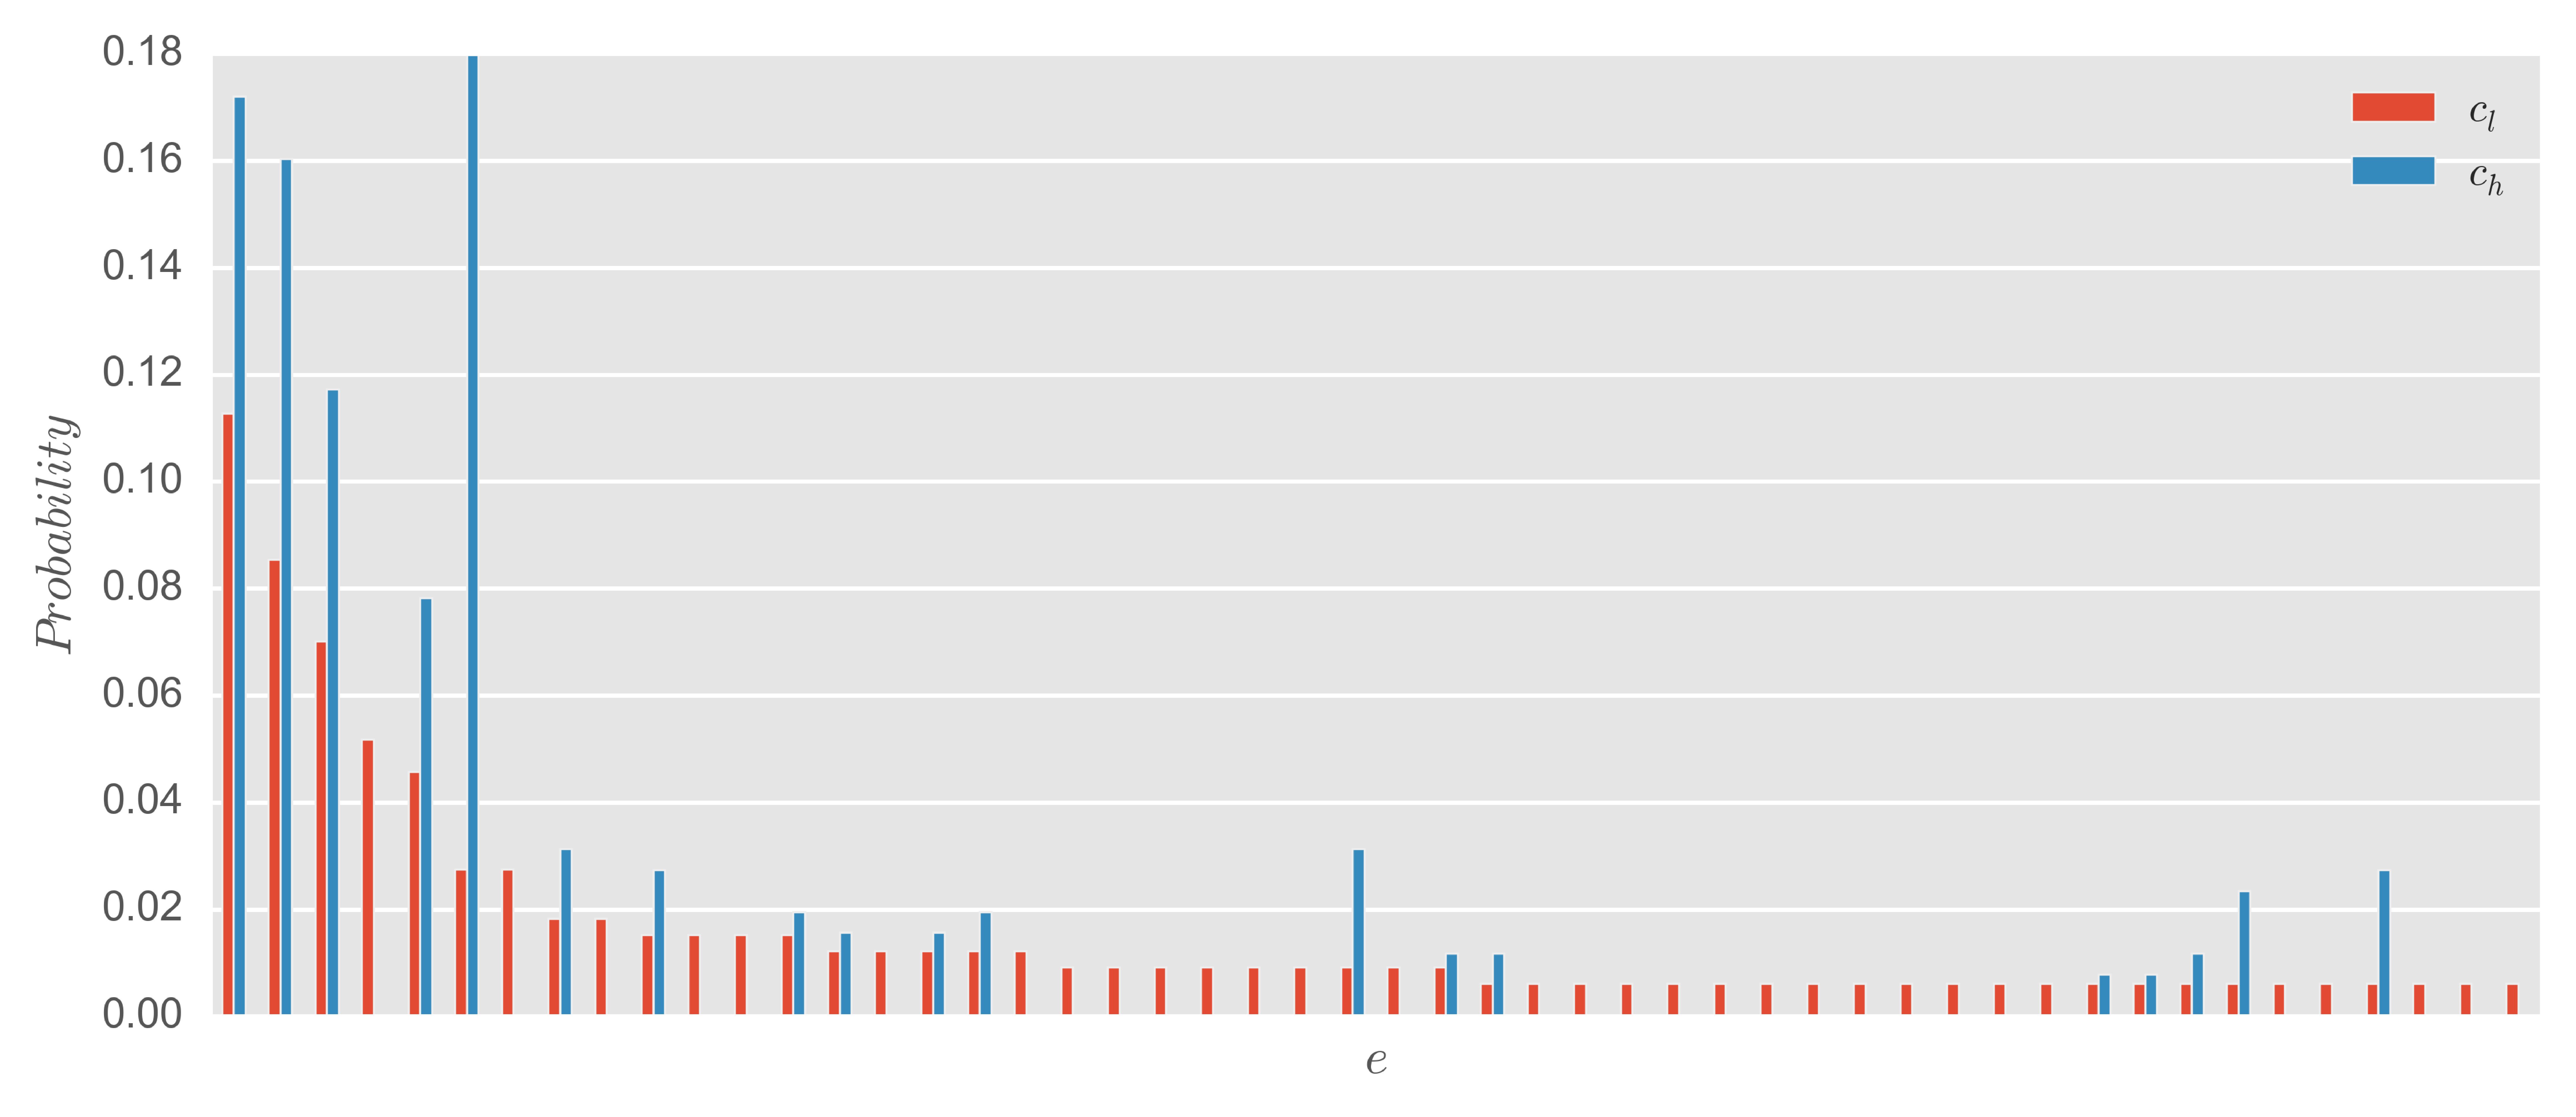
\epsfig{file=resources/df_hac_50_bill_gates.eps,width=\columnwidth}
\caption{Comparison between distribution of head aggregation and original Probase for \at{Bill Gates}. \small The red bars means $P(c|e)$ and the blue ones represents $p(h|e)$. Only top 50 concepts are shown due to space limit.  }
\label{fig:hac}
\end{figure}


\xch{not really need to be similar with the original, but I will do it}. We report the Pearson correlation between....

We further give case studies in Table.~\ref{tab:rerank} with the comparison to the direct estimation of $P(c|e)$ using Probase. 
%
%\begin{table*}[htbp!]
%  \centering
%  \caption{Rerank comparation}
%    \begin{tabular}{llrrlrr}
%    \toprule
%    \multicolumn{1}{c}{} & \multicolumn{3}{c}{aggregated} & \multicolumn{3}{c}{original head concepts} \\
%    \midrule
%    \multicolumn{1}{c}{Entity} & agg head & agg count & agg prob & org head & org count & org prob \\
%    \midrule
%    \multicolumn{1}{c}{\multirow{10}[0]{*}{shanghai}} & city  & 1311  & 0.829222 & city  & 644   & 0.407337 \\
%    \multicolumn{1}{c}{} & region & 46    & 0.029096 & region & 27    & 0.017078 \\
%    \multicolumn{1}{c}{} & area  & 42    & 0.026565 & metropolis & 23    & 0.014548 \\
%    \multicolumn{1}{c}{} & metropolis & 26    & 0.016445 & megacities & 15    & 0.009488 \\
%    \multicolumn{1}{c}{} & port  & 20    & 0.01265 & market & 15    & 0.009488 \\
%    \multicolumn{1}{c}{} & market & 19    & 0.012018 & location & 15    & 0.009488 \\
%    \multicolumn{1}{c}{} & centre & 18    & 0.011385 & port  & 9     & 0.005693 \\
%    \multicolumn{1}{c}{} & location & 17    & 0.010753 & locality & 6     & 0.003795 \\
%    \multicolumn{1}{c}{} & megacities & 15    & 0.009488 & locale & 5     & 0.003163 \\
%    \multicolumn{1}{c}{} & center & 11    & 0.006958 & seaport & 4     & 0.00253 \\
%          &       &       &       &       &       &  \\
%    \multicolumn{1}{c}{\multirow{10}[0]{*}{bill gates}} & leader & 46    & 0.140244 & billionaire & 37    & 0.112805 \\
%    \multicolumn{1}{c}{} & billionaire & 44    & 0.134146 & entrepreneur & 28    & 0.085366 \\
%    \multicolumn{1}{c}{} & entrepreneur & 41    & 0.125 & philanthropist & 23    & 0.070122 \\
%    \multicolumn{1}{c}{} & philanthropist & 30    & 0.091463 & celebrity & 15    & 0.045732 \\
%    \multicolumn{1}{c}{} & celebrity & 20    & 0.060976 & leader & 9     & 0.027439 \\
%    \multicolumn{1}{c}{} & person & 16    & 0.04878 & innovator & 6     & 0.018293 \\
%    \multicolumn{1}{c}{} & figure & 11    & 0.033537 & personality & 5     & 0.015244 \\
%    \multicolumn{1}{c}{} & innovator & 8     & 0.02439 & expert & 5     & 0.015244 \\
%    \multicolumn{1}{c}{} & luminary & 8     & 0.02439 & folks & 4     & 0.012195 \\
%    \multicolumn{1}{c}{} & individual & 7     & 0.021341 & icon  & 4     & 0.012195 \\
%          &       &       &       &       &       &  \\
%    \multicolumn{1}{c}{\multirow{10}[0]{*}{samsung}} & company & 1030  & 0.376875 & company & 816   & 0.298573 \\
%    \multicolumn{1}{c}{} & brand & 829   & 0.30333 & brand & 561   & 0.205269 \\
%    \multicolumn{1}{c}{} & manufacturer & 238   & 0.087084 & client & 42    & 0.015368 \\
%    \multicolumn{1}{c}{} & maker & 112   & 0.040981 & firm  & 39    & 0.01427 \\
%    \multicolumn{1}{c}{} & player & 60    & 0.021954 & rival & 38    & 0.013904 \\
%    \multicolumn{1}{c}{} & phone & 60    & 0.021954 & player & 33    & 0.012075 \\
%    \multicolumn{1}{c}{} & giant & 51    & 0.018661 & phone & 30    & 0.010977 \\
%    \multicolumn{1}{c}{} & firm  & 49    & 0.017929 & conglomerate & 19    & 0.006952 \\
%    \multicolumn{1}{c}{} & name  & 49    & 0.017929 & corporation & 19    & 0.006952 \\
%    \multicolumn{1}{c}{} & conglomerate & 42    & 0.015368 & partner & 12    & 0.004391 \\
%          &       &       &       &       &       &  \\
%    \multicolumn{1}{c}{\multirow{10}[0]{*}{mona lisa}} & painting & 56    & 0.4   & painting & 33    & 0.235714 \\
%    \multicolumn{1}{c}{} & masterpiece & 21    & 0.15  & masterpiece & 16    & 0.114286 \\
%    \multicolumn{1}{c}{} & work  & 20    & 0.142857 & work  & 10    & 0.071429 \\
%    \multicolumn{1}{c}{} & film  & 6     & 0.042857 & film  & 5     & 0.035714 \\
%    \multicolumn{1}{c}{} & image & 5     & 0.035714 & image & 3     & 0.021429 \\
%    \multicolumn{1}{c}{} & artwork & 4     & 0.028571 & picture & 3     & 0.021429 \\
%    \multicolumn{1}{c}{} & portrait & 4     & 0.028571 & treasure & 2     & 0.014286 \\
%    \multicolumn{1}{c}{} & piece & 4     & 0.028571 & song  & 2     & 0.014286 \\
%    \multicolumn{1}{c}{} & picture & 3     & 0.021429 & icon  & 2     & 0.014286 \\
%    \multicolumn{1}{c}{} & figure & 3     & 0.021429 & artwork & 1     & 0.007143 \\
%    \bottomrule
%
%    \end{tabular}%
%  \label{tab:rerank}%
%\end{table*}%



%\subsection{Find alias}

%\subsubsection{compare}
%
%In this section we compare $ P(<c_1,c_2 >|a )$ with $ P(c_1|a) \times P(c_2|a)$ to show that

\subsection{Exp 3: Joint Conceptualization}
Now, we evaluate the effectiveness of joint conceptualization, which is implemented by the introduction of $\alpha(c_1,c_2)$ in Eq.~\ref{eq:target_expand2_jr}. 
We compare to the baseline method in Eq~\ref{eq:naive}.
We present Table~\ref{tab:expjc} to show many cases where $\alpha$ help identify the true concept pair (ranked as the first).
Due to space limit, we place the entity with multiple meaning at $e_1$ and present result of $c_1$ only.
\begin{table}[htbp]
  \centering
  \caption{Joint Conceptualization with and without $\alpha$}
    \begin{tabular}{rrrr}
    \toprule
    $e_1$                               & $e_2$                               & $c_1 $  without $\alpha$       & $c_1$  with $\alpha$ \\
    \midrule
    columbia                            & barack obama                        & country                    & \textbf{school }\\
    apple                               & steve jobs                          & fruit                & \textbf{company} \\
   da vinci code           & ron howard                       & book                     & \textbf{film} \\
    spa                                 & belgium                             & facility                  & \textbf{place} \\
    \bottomrule
    \end{tabular}%
  \label{tab:expjc}%
\end{table}%



%
%{\bf Since there are many entities belongs to the same concept and we only consider topK $(c_1,c_2)$ pairs that has high typicality $P( (c_1,c_2) |a)$, so that the weird $(c_1,c_2)$ patterns as manifest in Example.~\ref{exa:sd} can be easily filtered.}
%
%\begin{figure}[!htb]
%\centering 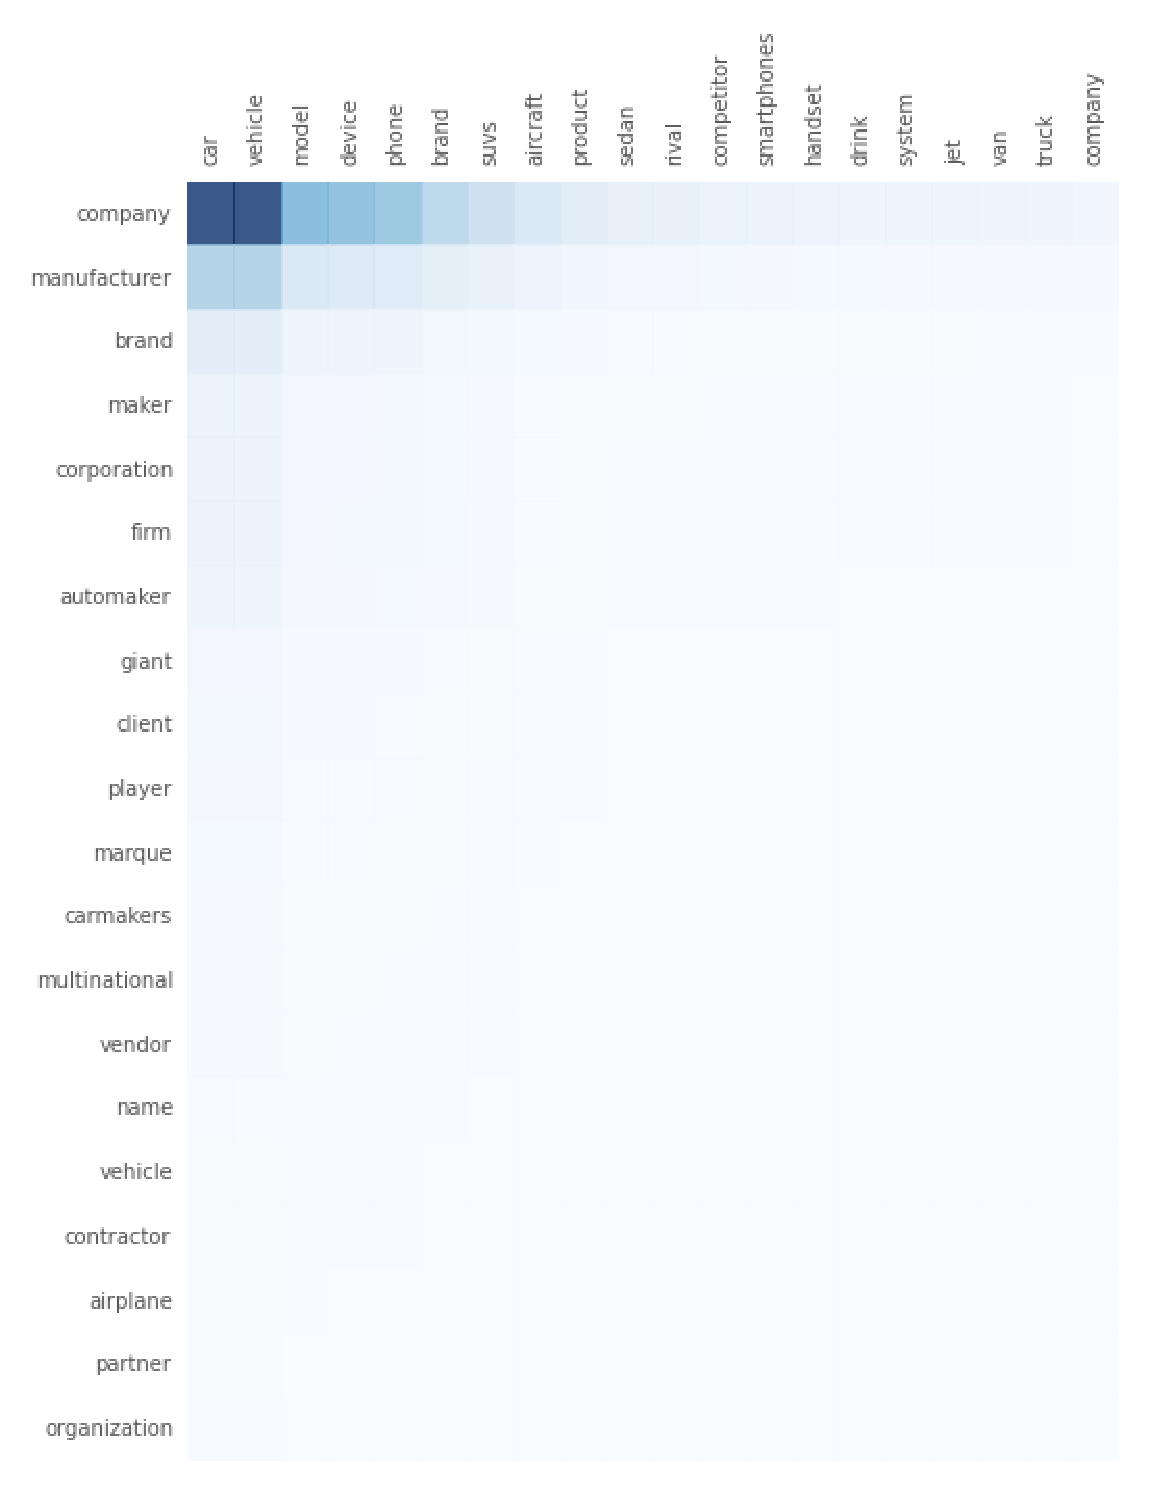
\epsfig{file=resources/ev_plot_manufacturer.eps,width=2.5in}
%\caption{$(c_1,c_2$) plot for attribute \term{Manufacturer}. } \label{fig:evplot}
%\end{figure}
%
%\begin{example}[Sense Disambiguation]
%Consider the following $(e1,a,e2)$ tuple \term{(iphone, manufacturer, apple)}. Suppose it is our query, where \term{apple}'s sense can either be a kind of \term{fruit} or a \term{company}.
%Fig.~\ref{fig:evplot} is a heatmap for all the concepts pairs $(c_1,c_2)$ of attributes \term{manufacturer}. The horizontal axis represents the $e_1$ and the vertical axis stands for $e_2$. The darker the blue is, the higher typicality it will be. In Fig.~\ref{fig:evplot}, We can observe that the top concepts of $e_2$ in the heatmap are \term{company, manufacturer,...} and top 10 pairs also does not include \term{fruit}. The intuition for this is that there exists thousands of $(e1,a,e2)$ tuple such as \term{(BMW\_Z4,manufacturer,BMW),(PlayStation\_4,manufacturer,Sony)} other than \term{(iphone, manufacturer, apple)} tuple, which results in a reasonable distribution.
%\label{exa:sd}
%\end{example}
%
%We further present a comparison of Eq.~\ref{eq:target_expand2_jr} and Eq.~\ref{eq:target_expand2_naive}, where the conceptualization is done with and without multiplying $\alpha(c_1,c_2)$.
%
%\begin{figure}[!htb]
%\centering
%\epsfig{file=resources/df_for_plot_foundedBy.eps,width=\columnwidth }
%\caption{Distribution of $P(\langle c_1,c_2 \rangle|\langle e_1,e_2 \rangle )$ of attribute \at{foundedBy} \textbf{without} $\alpha$. }
%\label{fig:c1c2}
%\end{figure}
%
%\begin{figure}[!htb]
%\centering
%\epsfig{file=resources/df_for_plot_foundedBy_with_alpha_c1c2.eps,width=\columnwidth}
%\caption{Distribution of $P(\langle c_1,c_2 \rangle|\langle e_1,e_2 \rangle )$ of attribute \at{foundedBy} \textbf{with} $\alpha=P(\langle c_1,c_2 \rangle)$. }
%\label{fig:c1c2_alpha}
%\end{figure}
%
%\begin{figure}[!htb]
%\centering
%\epsfig{file=resources/df_for_plot_foundedBy_with_alpha.eps,width=\columnwidth}
%\caption{Distribution of $P(\langle c_1,c_2 \rangle|\langle e_1,e_2 \rangle )$ of attribute \at{foundedBy} \textbf{with} $\alpha=P(\langle c_1,c_2 \rangle|a)$. }
%\label{fig:c1c2_alpha_given_a}
%\end{figure}
%
%
%We present the visualization of the distribution of $P(\langle c_1,c_2 \rangle|\langle e_1,e_2 \rangle )$ for Eq.~\ref{eq:naive} in Figure~\ref{fig:c1c2} and for Eq.~\ref{eq:target_expand2_jr} in Figure~\ref{fig:c1c2_alpha}.
%The floats inside each box represents $P(\langle c_1,c_2 \rangle|\langle e_1,e_2 \rangle )$, when the pair $\langle c_1,c_2 \rangle$ does not exist, we add a small value to $\alpha$ and then do normalization for smoothing purpose.

Apparently, the result with $\alpha$ is significantly better. 
It removes the concept-level ambiguity, for instance \at{apple} as a \at{fruit}.


\subsection{Exp 4: Collective Conceptualization}
We compare our approach with an $MDL$ based collective conceptualization solution~\cite{sunconceptual}, which aims at generating a minimum set of conceptual labels that best summarize a bag of words.
In our case, the bag of words refers to entities.
$MDL$ use $\alpha$ to tune the balance between \ac{Minimality} and \ac{Coverage}. 
Bigger $\alpha$ lead to better coverage as well as high-level/general concepts.
We set the parameter $\alpha$ in $MDL$ to 0.5 for normal comparison and 0.1 for gaining more concept pairs.

In the experiment, we select 50 attributes from different relation groups (such as \ac{PERSON-ORGNIZATION, PERSON-AFFLIATION, OBJECT-LOCATION} etc.\ ) and manually evaluate the top 20 concept pairs for each attribute.
Volunteers evaluates \textbf{2} for excellent pairs(e.g. \at{<company, entrepreneur>} for \at{FoundedBy}), \textbf{1} for correct while not apropos ones (e.g. \at{<song, celebrity>} for \at{writer} ), while \textbf{0} for wrong concept pairs (e.g. \at{<topic, Country>} for \at{SpokenIn} )
We present the human evaluated score in Figure~\ref{fig:eva_violin_pc1c2ga}.

We also show the distribution information on each relation group produced by $ERF$ in Figure~\ref{fig:eva_violin_group}.

\begin{figure}[!htb]
\centering
\epsfig{file=resources/violin_eval.eps,width=1.1\columnwidth}
\caption{Distribution of Human Evaluated result for $P(\langle c_1,c_2 \rangle|a)$. \small The white part is metric@1 and the red part is metric@10. Dashed line means quartiles of the distribution. The $ERF$ in the middle is our result, compared with $MDL@\alpha=0.5$(left) and $MDL@\alpha=0.1$(right). }
\label{fig:eva_violin_pc1c2ga}
\end{figure}

The $nDCG@1$ score is reasonably low since the correct concept pair is often more than 1.
We can observe a significant increase in the $nDCG@10$ score in our approach while not much increase in $MDL$-based approach since $MDL$ tends to give as few concepts as possible and sacrifices the coverage when $\alpha$ is small.
The $ERR@1$ and $ERR@10$ mesure varies not that much due to its user-behavioral instinct, which pays less attention to the lower-ranked pairs when find the correct concept pair above.
The $ERF$ approach provides rich correct concept pairs to handle the long-tailed concept pairs and gain an slight increase in $ERR@10$

\begin{figure*}[!htb]
\centering
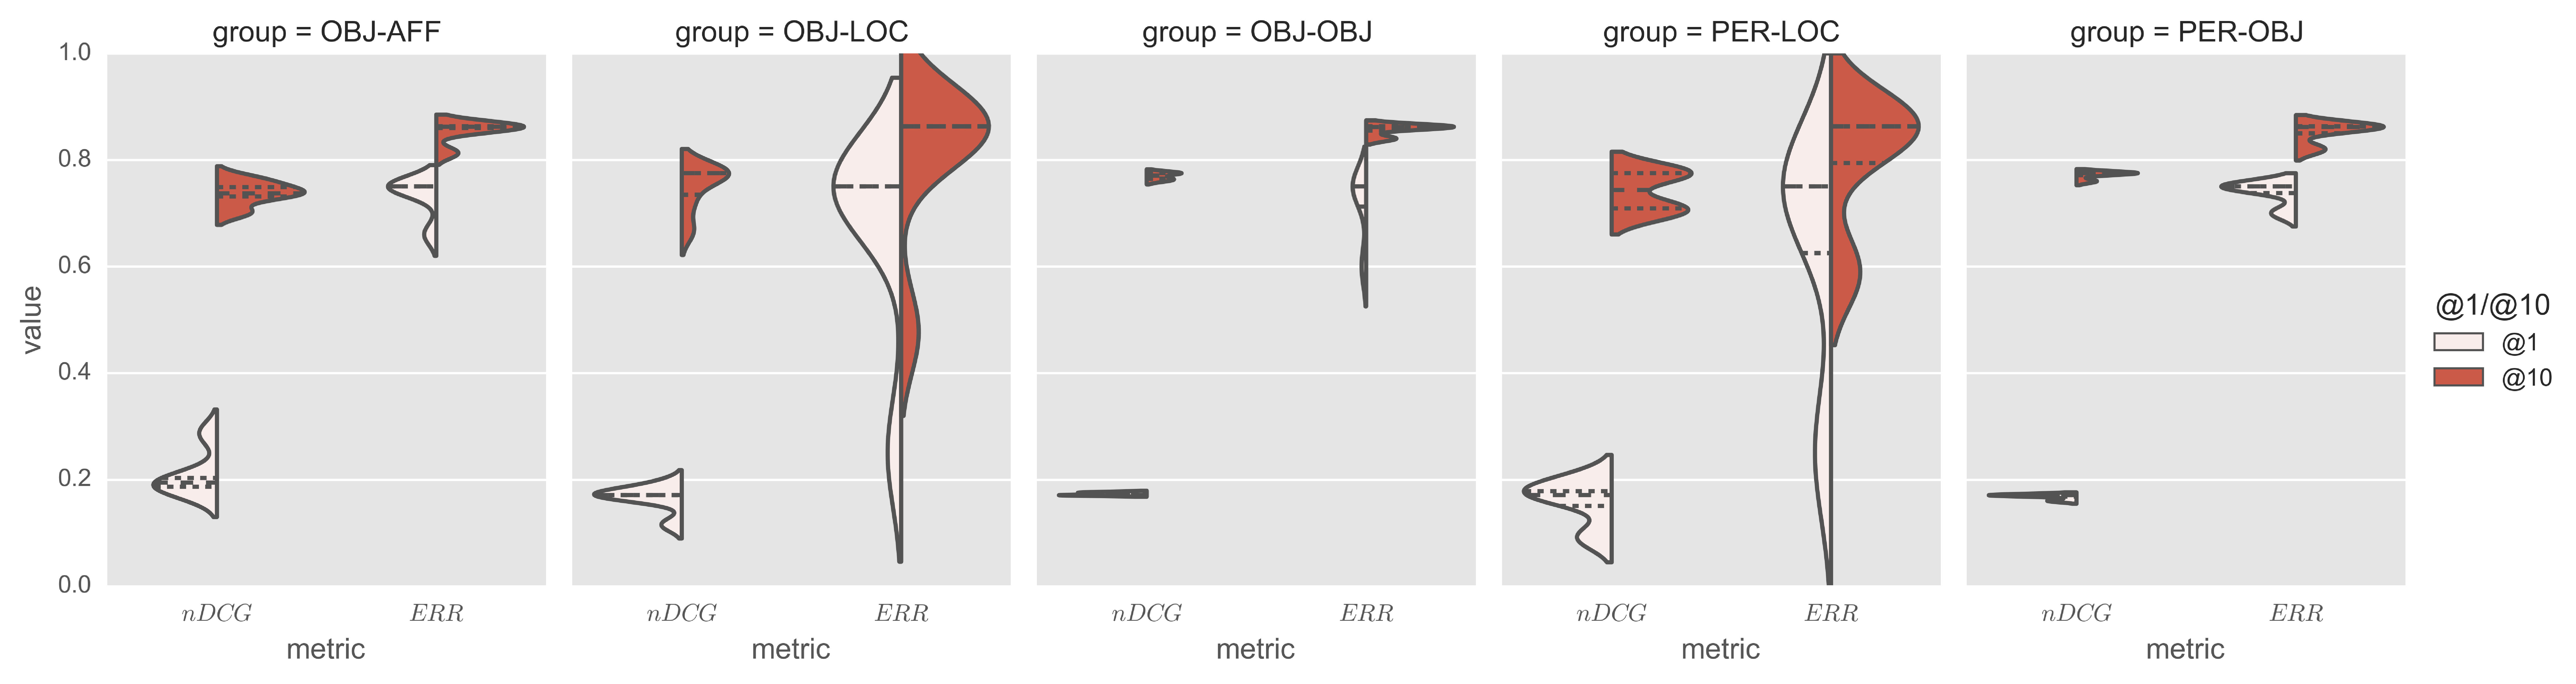
\epsfig{file=resources/violin_eval_group.eps,width=2.2\columnwidth}
\caption{Distribution of Human Evaluated result for $P(\langle c_1,c_2 \rangle|a)$ produced by $ERF$. \small Each seperate graph represents a relations group.}
\label{fig:eva_violin_group}
\end{figure*}



\subsection{Case Study}

We show some of the relations that has been retrieved by our method in Table~\ref{tab:results}.
The first 2 columns show the query entity pair.
The 3rd column is the relation retrieved by $ERF$ with a confidence score in the 4th column.
Note that we combine the relation of $\langle e_1,e_2\rangle$ and $\langle e_2,e_1\rangle$ into one single result.
For example the relation \at{commander} of \at{<adolf hitler,world war ii>} is actually that of \at{<world war ii, adolf hilter>}
% Table generated by Excel2LaTeX from sheet 'Sheet1'
\begin{table}[ht!]
  \centering
  \caption{First three results produced by ERF}
    \begin{tabular}{cccr}
    \toprule
    Entity1 & Entity2 & Relation & Score \\
    \midrule
    \multicolumn{1}{c}{\multirow{3}{*}{\parbox{1cm}{ Sherlock Holmes}}} & \multicolumn{1}{c}{\multirow{3}[0]{*}{united kingdom}} & anthem & 0.007079 \\
    \multicolumn{1}{c}{} & \multicolumn{1}{c}{} & firstAppearance & 0.004487 \\
    \multicolumn{1}{c}{} & \multicolumn{1}{c}{} & allegiance & 0.004357 \\
    \hline
    \multicolumn{1}{c}{\multirow{3}{*}{\parbox{1cm}{\centering apple}}} & \multicolumn{1}{c}{\multirow{3}[0]{*}{steve jobs}} & foundedBy & 0.015439 \\
    \multicolumn{1}{c}{} & \multicolumn{1}{c}{} & keyPerson & 0.009932 \\
    \multicolumn{1}{c}{} & \multicolumn{1}{c}{} & successor & 0.008069 \\
    \hline
    \multicolumn{1}{c}{\multirow{3}{*}{\parbox{1cm}{\centering Adolf Hitler}}} & \multicolumn{1}{c}{\multirow{3}[0]{*}{world war ii}} & commander & 0.037712 \\
    \multicolumn{1}{c}{} & \multicolumn{1}{c}{} & battle & 0.022161 \\
    \multicolumn{1}{c}{} & \multicolumn{1}{c}{} & ceo   & 2.44E-05 \\
    \hline
    \multicolumn{1}{c}{\multirow{3}{*}{\parbox{1cm}{\centering Microsoft}}} & \multicolumn{1}{c}{\multirow{3}[0]{*}{redmond}} & locationCity & 0.082507 \\
    \multicolumn{1}{c}{} & \multicolumn{1}{c}{} & foundationPlace & 0.047192 \\
    \multicolumn{1}{c}{} & \multicolumn{1}{c}{} & location & 0.036916 \\
    \hline
    \multicolumn{1}{c}{\multirow{3}{*}{Titanic}} & \multicolumn{1}{c}{\multirow{3}[0]{*}{James Cameron}} & director & 0.124407 \\
    \multicolumn{1}{c}{} & \multicolumn{1}{c}{} & cinematography & 0.096447 \\
    \multicolumn{1}{c}{} & \multicolumn{1}{c}{} & editing & 0.080134 \\
    \hline
    \multicolumn{1}{c}{\multirow{3}{*}{Titanic}} & \multicolumn{1}{c}{\multirow{3}[0]{*}{Leonardo Dicaprio}} & starring & 0.049689 \\
    \multicolumn{1}{c}{} & \multicolumn{1}{c}{} & narrator & 0.037267 \\
    \multicolumn{1}{c}{} & \multicolumn{1}{c}{} & producer & 0.01306 \\
    \hline
    \multicolumn{1}{c}{\multirow{3}{*}{\parbox{1cm}{\centering Harry Potter}}} & \multicolumn{1}{c}{\multirow{3}[0]{*}{J K rowling}} & notableWork & 0.016965 \\
    \multicolumn{1}{c}{} & \multicolumn{1}{c}{} & author & 0.015514 \\
    \multicolumn{1}{c}{} & \multicolumn{1}{c}{} & coverArtist & 0.014906 \\
    \bottomrule
    \end{tabular}%
  \label{tab:results}%
\end{table}%


%\subsection{Selectional Preference}

\section{Conclusion}
\label{sec:conclusion}

We studied the problem of explaining the relationship between two Wikipedia pages that are hyperlinked. 
If there exists a SPO triple explicitly explaining the relationship, this problem degenerates to the retrieval of such triple. 
However, we found such case is extremely rare, 1.5\%, and thus increasing recall for the rest pairs is crucial. We proposed to use concept pairs as intermediate variables to find a typical attribute for this pair as a possible explanation. We observed that, to ensure accuracy, such conceptualization should jointly optimize for both entities and identify head concepts. We validated our framework using real-life Wikipedia entities and taxonomies.


\bibliographystyle{abbrv}
\bibliography{refer}


\end{document}
